\begin{frame}{D-calculus: quan sát mạch tốt và mạch lỗi}
\centering
\begin{tabular}{c|cc}
Giá trị & Tốt & Lỗi\\\hline
$0$ & 0 & 0\\
$1$ & 1 & 1\\
$X$ & ? & ?\\
$D$ & 1 & 0\\
$\overline D$ & 0 & 1
\end{tabular}
\begin{block}{Tính cổng trên từng thành phần}
$D\land1=D$, $D\land\overline D=0$, $D\land X=X$.\\
Qua NAND với ngõ vào phụ bằng 1: $D\leftrightarrow\overline D$.
\end{block}
\end{frame}

\begin{frame}{Bảng logic năm giá trị cho tám loại cổng}
\centering\scriptsize
\renewcommand{\arraystretch}{1.05}
\setlength{\tabcolsep}{3pt}
\begin{minipage}[t]{0.24\textwidth}\centering
\textbf{AND}\\[1pt]
\begin{tabular}{@{}c|ccccc@{}}
$a\backslash b$ & 0 & 1 & $X$ & $D$ & $\overline{D}$\\\hline
0 & 0 & 0 & 0 & 0 & 0\\
1 & 0 & 1 & $X$ & $D$ & $\overline{D}$\\
$X$ & 0 & $X$ & $X$ & $X$ & $X$\\
$D$ & 0 & $D$ & $X$ & $D$ & 0\\
$\overline{D}$ & 0 & $\overline{D}$ & $X$ & 0 & $\overline{D}$\\
\end{tabular}
\end{minipage}\hfill
\begin{minipage}[t]{0.24\textwidth}\centering
\textbf{NAND}\\[1pt]
\begin{tabular}{@{}c|ccccc@{}}
$a\backslash b$ & 0 & 1 & $X$ & $D$ & $\overline{D}$\\\hline
0 & 1 & 1 & 1 & 1 & 1\\
1 & 1 & 0 & $X$ & $\overline{D}$ & $D$\\
$X$ & 1 & $X$ & $X$ & $X$ & $X$\\
$D$ & 1 & $\overline{D}$ & $X$ & $\overline{D}$ & 1\\
$\overline{D}$ & 1 & $D$ & $X$ & 1 & $D$\\
\end{tabular}
\end{minipage}\hfill
\begin{minipage}[t]{0.24\textwidth}\centering
\textbf{OR}\\[1pt]
\begin{tabular}{@{}c|ccccc@{}}
$a\backslash b$ & 0 & 1 & $X$ & $D$ & $\overline{D}$\\\hline
0 & 0 & 1 & $X$ & $D$ & $\overline{D}$\\
1 & 1 & 1 & 1 & 1 & 1\\
$X$ & $X$ & 1 & $X$ & $X$ & $X$\\
$D$ & $D$ & 1 & $X$ & $D$ & 1\\
$\overline{D}$ & $\overline{D}$ & 1 & $X$ & 1 & $\overline{D}$\\
\end{tabular}
\end{minipage}\hfill
\begin{minipage}[t]{0.24\textwidth}\centering
\textbf{NOR}\\[1pt]
\begin{tabular}{@{}c|ccccc@{}}
$a\backslash b$ & 0 & 1 & $X$ & $D$ & $\overline{D}$\\\hline
0 & 1 & 0 & $X$ & $\overline{D}$ & $D$\\
1 & 0 & 0 & 0 & 0 & 0\\
$X$ & $X$ & 0 & $X$ & $X$ & $X$\\
$D$ & $\overline{D}$ & 0 & $X$ & $\overline{D}$ & 0\\
$\overline{D}$ & $D$ & 0 & $X$ & 0 & $D$\\
\end{tabular}
\end{minipage}

\vspace{3mm}
\begin{minipage}[t]{0.24\textwidth}\centering
\textbf{XOR}\\[1pt]
\begin{tabular}{@{}c|ccccc@{}}
$a\backslash b$ & 0 & 1 & $X$ & $D$ & $\overline{D}$\\\hline
0 & 0 & 1 & $X$ & $D$ & $\overline{D}$\\
1 & 1 & 0 & $X$ & $\overline{D}$ & $D$\\
$X$ & $X$ & $X$ & $X$ & $X$ & $X$\\
$D$ & $D$ & $\overline{D}$ & $X$ & 0 & 1\\
$\overline{D}$ & $\overline{D}$ & $D$ & $X$ & 1 & 0\\
\end{tabular}
\end{minipage}\hfill
\begin{minipage}[t]{0.24\textwidth}\centering
\textbf{XNOR}\\[1pt]
\begin{tabular}{@{}c|ccccc@{}}
$a\backslash b$ & 0 & 1 & $X$ & $D$ & $\overline{D}$\\\hline
0 & 1 & 0 & $X$ & $\overline{D}$ & $D$\\
1 & 0 & 1 & $X$ & $D$ & $\overline{D}$\\
$X$ & $X$ & $X$ & $X$ & $X$ & $X$\\
$D$ & $\overline{D}$ & $D$ & $X$ & 1 & 0\\
$\overline{D}$ & $D$ & $\overline{D}$ & $X$ & 0 & 1\\
\end{tabular}
\end{minipage}\hfill
\begin{minipage}[t]{0.46\textwidth}\centering
\textbf{NOT}\\[1pt]
\begin{tabular}{@{}c|ccccc@{}}
vào & 0 & 1 & $X$ & $D$ & $\overline{D}$\\\hline
ra & 1 & 0 & $X$ & $\overline{D}$ & $D$\\
\end{tabular}
\\[4mm]
\textbf{BUFF}\\[1pt]
\begin{tabular}{@{}c|ccccc@{}}
vào & 0 & 1 & $X$ & $D$ & $\overline{D}$\\\hline
ra & 0 & 1 & $X$ & $D$ & $\overline{D}$\\
\end{tabular}
\end{minipage}

\vspace{2mm}
{\footnotesize Hàng: ngõ vào $a$; cột: ngõ vào $b$. Dùng làm dữ liệu kiểm thử chung, khớp chương trình 160/160 ô.}
\end{frame}

\begin{frame}{D-algorithm: chọn cube, lan truyền và justify}
\begin{itemize}
\item NAND $(a,b,z)$: cover $(0,X,1)$, $(X,0,1)$, $(1,1,0)$.
\item PDCF cho $z/SA0$: $(0,X,D)$ hoặc $(X,0,D)$.
\item PDC: $(D,1,\overline D)$; ngõ vào phụ bằng 1 cho sai khác đi qua.
\item Giao cube: $X\cap v=v$; yêu cầu xác định trái nhau gây xung đột.
\item D-frontier: đầu vào có sai khác, đầu ra còn $X$.
\item J-frontier: đầu ra đã gán, đầu vào chưa justify được.
\end{itemize}
\begin{block}{Điều kiện thành công}
Sai khác tới PO, mọi yêu cầu được justify và nhất quán.\\
Xung đột: quay lui, khôi phục trạng thái và thử cube khác.
\end{block}
\end{frame}

\begin{frame}{c17, 11/SA0: lan truyền và justification}
\centering
\begingroup
\def\pTwoCSeventeenWidth{0.86\linewidth}
% P2: tái sử dụng hình mach_c17.jpg do người dùng cung cấp, không vẽ lại.
% Wrapper dùng được từ report/main.tex và slides/main.tex.
% Hình thể hiện cube tổng quát hóa (X,1,0,X,X).
\IfFileExists{figures/common/mach_c17.jpg}{%
  \includegraphics[width=0.72\linewidth]{figures/common/mach_c17.jpg}%
}{%
  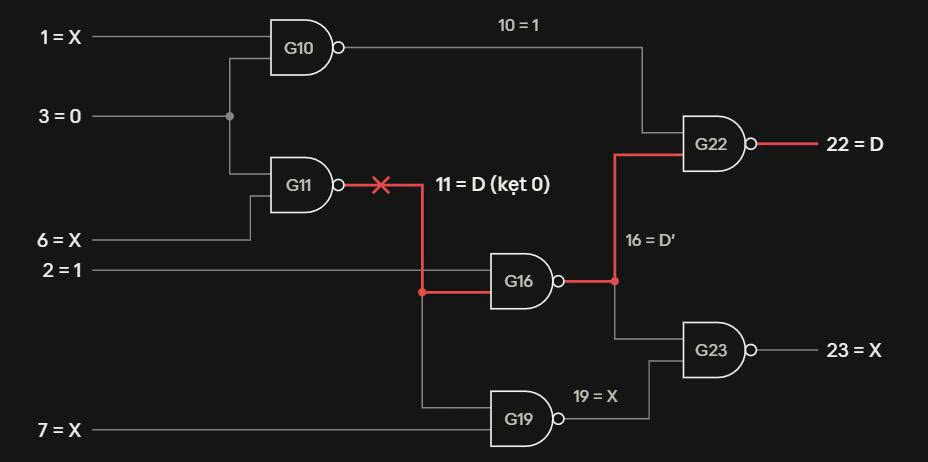
\includegraphics[width=0.72\linewidth]{../report/figures/common/mach_c17.jpg}%
}

\endgroup
\par\smallskip
\small
\begin{tabular}{clcl}
1 & PDCF: $6=0$, $11=D$ & 2 & PDC: $2=1$, $16=\overline D$\\
3 & PDC: $10=1$, $22=D$ & 4 & Justify: $3=0$, $J=\varnothing$
\end{tabular}
\par\smallskip
Cube gốc $(X,1,0,0,X)$; hình sau tổng quát hóa $(X,1,0,X,X)$.
\par
\footnotesize $X=0$: $01000$; PO tốt $(1,1)$, lỗi $(0,0)$.
4 lần chọn cube, 0 backtrack.
\end{frame}
